%!TEX program = xelatex
\documentclass[lang=cn,a4paper,newtx]{elegantpaper}

\title{ICU约束下流行病阈值控制策略分析}
\author{ XXX \and XXX}
\institute{School of Mathematics and Statistics, Shaanxi Normal University}
\version{0.1}
\date{\today}

\usepackage{amsmath,amssymb,mathrsfs}
\usepackage{booktabs}
\usepackage{graphicx}
\usepackage{float}
\usepackage{array}
\usepackage{tabularx}
\usepackage{multirow}
\usepackage{makecell}
\usepackage{threeparttable}
\usepackage{xurl}

\graphicspath{{../}{../figures/}{../table/}}
\numberwithin{equation}{section}
\allowdisplaybreaks[3]
\renewcommand{\arraystretch}{1.12}
\emergencystretch=2em

\begin{document}

\maketitle
\section{模型与医疗容量约束}
\subsection{包含追踪的SIR模型}
我们将人群划分为易感者 ($S$)、隔离中的易感者 ($S_q$)、非隔离感染者 ($I$)、隔离中的感染者 ($I_q$)、康复者 ($R$) 这几个仓室，我们记传播概率为 $\beta$，接触率为 $c(t)$。同时，我们将接触者追踪比例记为 $q(t)$，表示被追踪到的人群将根据其是否感染而被隔离（若易感则进入 $S_q$，若感染则进入 $I_q$）。同时，未被追踪到的人群（比例为 $1-q(t)$）是指暴露于病毒但被接触追踪遗漏的个体；如果他们被感染，将进入 $I$ 仓室。我们统一考虑$I$与$I_q$的康复者都进入同一个$R$仓室。两者的恢复率分别为 $\gamma$ 和 $\delta_q$。因此，系统的传播动态由以下方程组控制：       


\begin{equation}
\begin{cases}
\dfrac{dS(t)}{dt} = -\dfrac{\beta c(t) + c(t)q(t)(1-\beta)}{N} S(t)I(t), \\[.8em] % Add some space after the first line
\dfrac{dI(t)}{dt} = \dfrac{\beta c(t)(1-q(t))}{N} S(t)I(t)  - \gamma I(t), \\[.8em]
\dfrac{dS_q(t)}{dt} = \dfrac{(1-\beta)c(t)q(t)}{N} S(t)I(t), \\[.8em]
\dfrac{dI_q(t)}{dt} = \dfrac{\beta c(t) q(t)}{N} S(t)I(t) - \delta_q I_q(t), \\[.8em]
\dfrac{dR(t)}{dt} = \gamma I(t) + \delta_q I_q(t).
\end{cases}
\end{equation}

\begin{figure}[h]
    \centering
    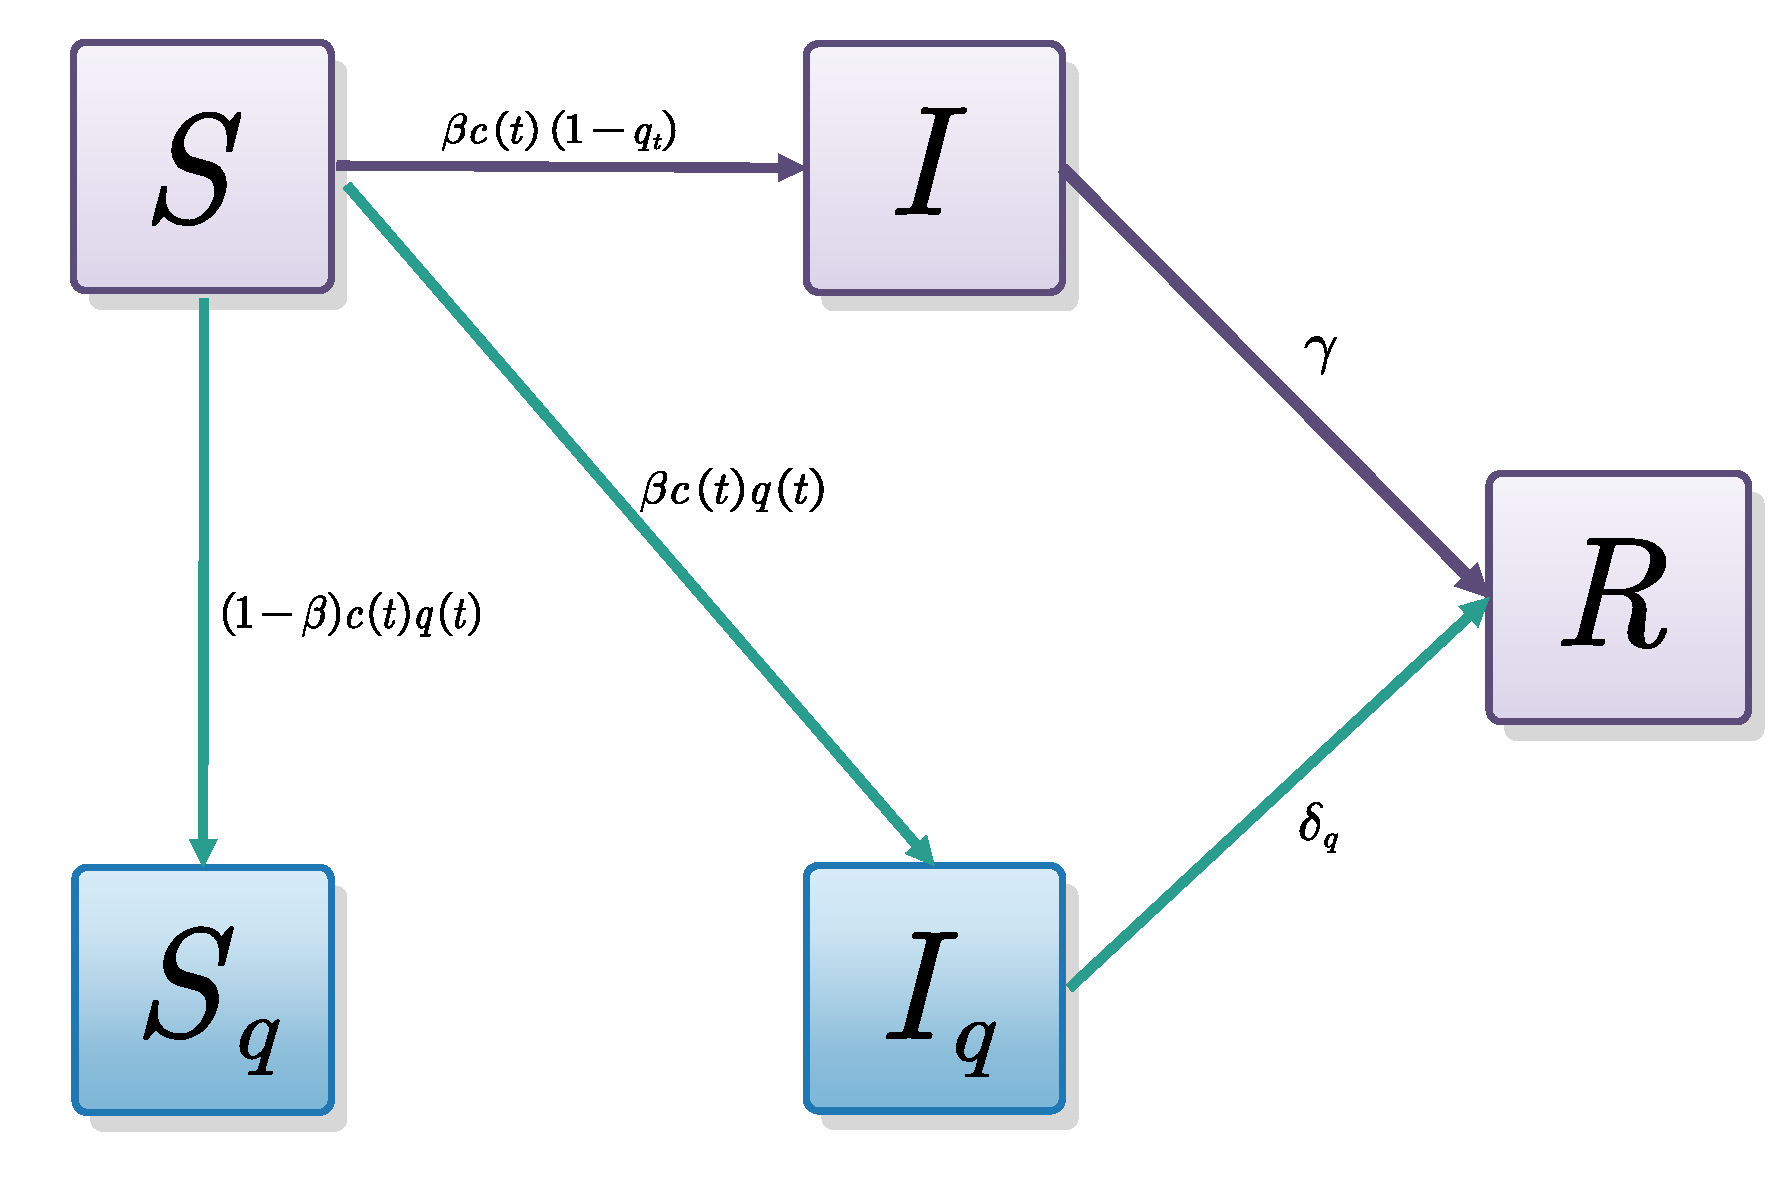
\includegraphics[width=0.8\textwidth]{figures/Fig1.pdf}
\end{figure}
\subsection{模型控制}
在传染病流行期间，如何设计控制策略以防止非隔离感染者($I$)数量超过重症监护室($ICU$)的数量，是一个重要的公共卫生问题。为解决这一关键问题，我们将控制策略引入到接触率 $c(t)$ 和隔离率 $q(t)$ 中。

我们假设控制分三个阶段：
\begin{itemize}
    \item 常规防控阶段 ($t<t_1$);
    \item 加强防控阶段 ($t_1 \leq t \leq t_2$);
    \item 常规防控阶段 ($t > t_2$).
\end{itemize}

相应地，我们令 $c_0$ 和 $q_0$ 分别表示常规防控阶段下的接触率和隔离率，其中 $c_0>0$、$0\le q_0<1$。为了避免符号混淆，记加强防控阶段采用的控制轨迹为 $c_c(t)$ 和 $q_c(t)$。一旦在 $t=t_1$ 时启动加强控制，系统由常规水平 $(c_0,q_0)$ 切换到加强轨迹 $(c_c(t),q_c(t))$；当 $t=t_2$ 时解除加强控制，系统恢复到常规防控水平 $(c_0,q_0)$。因此，一个作用于系统的控制方案可以表述如下：
\begin{equation}
c(t) = 
\begin{cases} 
c_0, & t < t_1, \\
c_c(t), & t_1 \leq t \leq t_2, \\
c_0, & t > t_2, 
\end{cases}
\quad \text{and} \quad 
q(t) = 
\begin{cases} 
q_0, & t < t_1, \\
q_c(t), & t_1 \leq t \leq t_2, \\
q_0, & t > t_2. 
\end{cases}
\label{eq:model:piecewise-control}
\end{equation}

传统的控制策略通常通过持续性限制措施降低各时段的瞬时感染人数，从而压低感染峰值。然而，持续性强限制不仅难以长期维持，也会对正常社会生活和经济活动造成影响。因此，本文关注一种“精确压平曲线”理想控制策略：在不预设最优控制成本泛函的前提下，将 $I(t)\le \eta$ 作为医疗容量硬约束，并在系统首次触及红线后施加刚好使 $\dot I=0$ 的加强控制。


\textbf{策略定义}：设定ICU的医疗资源上限为 $I(t) \le \eta$。社会规划者的策略阶段定义为：
\begin{enumerate}
    \item \textbf{前期常规控制 ($0 \le t < t_1$)}：系统在背景防控水平 $(c_0,q_0)$ 下演化，直至$I$首次触碰容量上限 $\eta$。
    \item \textbf{中期加强控制 ($t_1 \le t \le t_2$)}：启动并动态调节加强控制 $(c_c(t),q_c(t))$，施加刚好的控制力使得$I$严格维持在天花板（$\dot{I}=0, I=\eta$），直至$S$降至背景防控水平下的临界阈值。
    \item \textbf{后期恢复常规控制 ($t > t_2$)}：系统跨越背景临界点，疫情进入自然衰退期，解除加强控制并恢复到 $(c_0,q_0)$。
\end{enumerate}

针对我们的控制策略，对于给定初值$(S_0, I_0)$，我们设在$t \in [0, t_1)$期间系统以常规防控水平演化，即$c(t) = c_0$,$q(t) = q_0$。在$t = t_1$时刻，系统首次触碰医疗上限，即 $I(t_1) = \eta$。令此时对应的易感人数（干预启动阈值）为 $S^* = S(t_1)$。

在控制期间 $t \in [t_1, t_2]$ 内，为精准维持 $I(t) \equiv \eta$，系统的演化必须满足条件 $\dot{I} = 0$，此时的控制为 $c_c(t)$ 和 $q_c(t)$。

设在$t = t_2$时刻，解除加强控制，此时易感人数下降到常规防控水平下的临界阈值：
\begin{equation}
S(t_2)=S_c\doteq \frac{ \gamma N}{\beta c_0(1-q_0)}.
\end{equation}
当$t > t_2$系统跨越该临界点，进入常态防控下的衰退期。此时的控制为$c(t)=c_0$,$q(t)=q_0$。


因此，我们的分析将围绕以下核心问题展开：
\begin{itemize}
    \item 解析求解干预启动点 $S^*$ 与时间 $t_1$；
    \item 推导阈值控制期的动态控制律 $c_c(t)$和$q_c(t)$ ；
    \item 推导阈值控制期的时间演化 $S(t)$ 和 控制结束时间 $t_2$；
    \item 分析这样的控制策略的效果，即分析时间演化 $S(t)$ 和 $I(t)$。以及参数对控制策略的影响。                                                   
\end{itemize}


\section{常规阶段首次积分与触发条件}
由于恢复者 $R$、隔离易感者 $S_q$ 和隔离感染者 $I_q$ 仓室与(1)中的前两个方程是解耦的，因此我们只需要考虑以下的二维系统
\begin{equation}
\begin{cases}
\dot{S}(t) = - \beta_1(t) S(t) I(t) \\
\dot{I}(t) =   \beta_2(t) S(t) I(t) - \gamma I(t)
\end{cases}
\label{eq:model:reduced-si}
\end{equation}
其中
\begin{equation}
\beta_1(t)=\frac{c(t)\big[\beta+q(t)(1-\beta)\big]}{N},
\qquad
\beta_2(t)=\frac{\beta c(t)(1-q(t))}{N}.
\label{eq:model:beta12-general}
\end{equation}
这里 $\gamma$ 表示非隔离感染者 $I$ 的移出率。按照式 \eqref{eq:model:piecewise-control}，三阶段控制可等价写成
\begin{equation}
\beta_i(t)=
\begin{cases}
\beta_i^0, & t<t_1,\\
\beta_i^1(t), & t_1\le t\le t_2,\\
\beta_i^0, & t>t_2,
\end{cases}
\qquad i=1,2,
\end{equation}
其中常规防控阶段的系数为
\begin{equation}
\beta_1^0=\frac{c_0\big[\beta+q_0(1-\beta)\big]}{N},
\qquad
\beta_2^0=\frac{\beta c_0(1-q_0)}{N}.
\label{eq:model:beta12-baseline}
\end{equation}
加强防控阶段的 $\beta_1^1(t)$ 与 $\beta_2^1(t)$ 则由具体情景中的控制轨迹 $c_c(t)$、$q_c(t)$ 决定。

当 $\beta_1$ 与 $\beta_2$ 为常数时，特别是在前期和后期的常规防控阶段，可以通过消去时间变量得到首次积分。为统一记号，定义
\begin{equation}
\rho_1=\frac{\gamma}{\beta_1^0},
\qquad
S_c=\frac{\gamma}{\beta_2^0}
=\frac{\gamma N}{\beta c_0(1-q_0)}.
\label{eq:model:baseline-symbols}
\end{equation}
并在情景一中记
\begin{equation}
\bar S=\frac{\gamma N(1-\beta)}{\beta c_0}<S_c.
\label{eq:s1:barS}
\end{equation}
其中 $S_c$ 是常规防控水平 $(c_0,q_0)$ 下的临界易感人数。给定初始状态 $(S_0,I_0)$，常规防控阶段的首次积分为
\begin{equation}
I(t)+\frac{\beta_2^0}{\beta_1^0} S(t)-\rho_1\ln S(t)
=
I_0+\frac{\beta_2^0}{\beta_1^0} S_0-\rho_1\ln S_0
\doteq C_0.
\label{eq:model:first-integral}
\end{equation}

为了确定干预策略的关键时间节点与对应的人口状态，需利用首次积分来求解临界易感人数$S^*$及其对应的首次到达时间$t_1$，以及通过$[t_1,t_2]$这段时间$I(t) = \eta(\dot{I}=0)$去计算$S(t),t \in [t_1,t_2]$和结束时间$t_2$以及控制函数$q_c(t)$,$c_c(t)$。

\section{情景一：$c(t) \equiv c_0$,只加强$q$控制}
本情景考虑在常规防控水平 $(c_0,q_0)$ 的基础上，不进一步调节接触率 $c(t)$，而只通过提高隔离率 $q(t)$ 来维持医疗红线。也就是说，整个过程中
\begin{equation*}
c(t)=c_0,\qquad t\ge 0,
\end{equation*}
而隔离率在前期和后期保持常规水平 $q_0$，只在加强控制期内切换为动态加强隔离率 $q_c(t)$。

此时动力系统为：
\begin{equation}
\begin{cases}
\dot{S}(t) = - \beta_1(t) S(t) I(t) \\
\dot{I}(t) = \beta_2(t) S(t) I(t) - \gamma I(t)
\end{cases}
\label{eq:s1:dynamics}
\end{equation}
其中
\begin{equation}
\beta_i(t)=
\begin{cases}
\beta_i^0, & t<t_1,\\
\beta_i^1(t), & t_1\le t\le t_2,\\
\beta_i^0, & t>t_2,
\end{cases}
\quad i=1,2,
\end{equation}
其中$\beta_1^0$和$\beta_2^0$由式 \eqref{eq:model:beta12-baseline} 给出
\begin{equation}
\beta_1^1(t)=\frac{c_0\big[\beta+q_c(t)(1-\beta)\big]}{N},
\quad
\beta_2^1(t)=\frac{\beta c_0(1-q_c(t))}{N}.
\label{eq:s1:beta12-control}
\end{equation}

\subsection{干预启动点 $S^*$ 与时间 $t_1$ }
\begin{theorem}
    对于系统 \eqref{eq:s1:dynamics}，在常规防控阶段 $t<t_1$，首次触碰医疗阈值的易感人数 $S^*$为：
    \begin{equation}
        S^*=-S_cW_{-1}\left(-\frac{1}{S_c}\exp\left[-\frac{C_0-\eta}{\rho_1}\right]\right)
        \label{eq:s1:Sstar-lambert}
    \end{equation}
    开始控制的时间$t_1$为:
    \begin{equation}
    t_1
    =
    \int_{S_0}^{S^*}
    \frac{1}{
    -\beta_1^0S\left[
    C_0-\frac{\beta_2^0}{\beta_1^0}S+\rho_1\ln S
    \right]
    }\,dS.
    \label{eq:s1:t1}
    \end{equation}
\end{theorem}
\begin{proof}
    在加强控制启动前，系统处于常规防控阶段，即 $c(t)=c_0$ 且 $q(t)=q_0$。
可得常规防控阶段的首次积分
\begin{equation}
I(t)+\frac{\beta_2^0}{\beta_1^0}S(t)-\rho_1\ln S(t)
=
I_0+\frac{\beta_2^0}{\beta_1^0}S_0-\rho_1\ln S_0
= C_0.
\label{eq:s1:first-integral}
\end{equation}

已知 $I(t_1)=\eta$，$S^*=S(t_1)$。将该边界条件代入式 \eqref{eq:s1:first-integral} 得
\[
\frac{\beta_2^0}{\beta_1^0}S^*-\rho_1\ln S^*
=C_0-\eta.
\]
这构成了关于 $S^*$ 的非线性超越方程。为了利用 Lambert $W$ 函数求解，注意到
\[
\frac{\beta_2^0}{\beta_1^0\rho_1}
=
\frac{\beta_2^0}{\gamma}
=
\frac{1}{S_c}.
\]
于是上式可化为
\[
-\frac{1}{S_c}S^*
\exp\left(-\frac{1}{S_c}S^*\right)
=
-\frac{1}{S_c}
\exp\left[-\frac{C_0-\eta}{\rho_1}\right].
\]
由于我们关注的是感染人数上升阶段首次触碰医疗红线，此时 $S^*>S_c$，故应选取 Lambert $W$ 函数的 $-1$ 分支：
\[
S^*
=
-\frac{\gamma N}{\beta c_0(1-q_0)}W_{-1}\left(
-\frac{\beta c_0(1-q_0)}{\gamma N}
\exp\left[-\frac{C_0-\eta}{\frac{\gamma}{\beta_1^0}}\right]
\right)
=
-S_c
W_{-1}\left(
-\frac{1}{S_c}
\exp\left[-\frac{C_0-\eta}{\rho_1}\right]
\right)
\]

在确定状态阈值 $S^*$ 后，启动加强控制的具体时间 $t_1$ 可由常规防控阶段的易感者的动态方程积分得到。由式 \eqref{eq:s1:first-integral} 有
\[
I(S)=
C_0-\frac{\beta_2^0}{\beta_1^0}S+\rho_1\ln S,
\]
因此
\[
t_1
=
\int_{S_0}^{S^*}
\frac{1}{
-\beta_1^0S\left[
C_0-\frac{\beta_2^0}{\beta_1^0}S+\rho_1\ln S
\right]
}\,dS.
\]
该定积分可通过数值求积求解。
\end{proof}

\begin{remark}
    ICU阈值能被触碰的条件是：$I_{\max}^{no} > \eta$,且为了问题有意义要求 $I_0 \le \eta$。其中 $I_{\max}^{no}$ 表示系统在常规防控水平 $(c_0,q_0)$ 下的感染峰值。具体地，在常规防控轨道上
    \begin{equation*}
    I(S)=I_0+\frac{\beta_2^0}{\beta_1^0}(S_0-S)+\rho_1\ln\frac{S}{S_0},
    \end{equation*}
    感染峰值发生在 $\dot I=0$，即 $S=S_c$ 处。因此
    \begin{equation}
    I_{\max}^{no}
    =
    I_0+\frac{\beta_2^0}{\beta_1^0}(S_0-S_c)
    +\rho_1\ln\frac{S_c}{S_0}.
    \label{eq:s1:Imax-no}
    \end{equation}
    如果 $I_{\max}^{no}\le \eta$，则常规防控已经足以避免突破医疗红线，无需启动加强控制；如果 $I_0>\eta$，则系统初始状态已经突破医疗红线。
\end{remark}

\subsection{阈值控制期的状态反馈控制 $q_c(S(t))$}
\begin{theorem}[阈值控制期的状态反馈律及其结构性质]
\label{thm:s1:qc-structure}
对系统\eqref{eq:s1:dynamics}，在阈值控制期 $t\in[t_1,t_2]$ 内精准维持 $I(t)\equiv\eta$（即 $\dot I=0$）所需的隔离强度由如下状态反馈律唯一确定：
\begin{equation}
q_c(t)=q_c(S(t))=1-\frac{\gamma N}{\beta c_0 S(t)} \quad S\in [S_c,S^*].
\label{eq:s1:q-control}
\end{equation}
从而完整的隔离控制律为
\begin{equation}
q(t)=
\begin{cases}
q_0, & t<t_1,\\
q_c(t)=1-\dfrac{\gamma N}{\beta c_0 S(t)}, & t_1\le t\le t_2,\\
q_0, & t>t_2.
\end{cases}
\label{eq:s1:q-piecewise}
\end{equation}
进一步地，设加强控制确实被触发，即 $S^*>S_c$（等价于 $I_0<\eta<I_{\max}^{no}$，见\eqref{eq:s1:Imax-no}后的注），则该控制律具有以下结构：
\begin{itemize}
\item[(i)] \textbf{瞬时启动}：$q(t)$ 在 $t=t_1$ 处发生向上跳跃间断，
\[
q(t_1^-)=q_0<q(t_1)=q_{\max}=1-\frac{\gamma N}{\beta c_0 S^*},
\qquad
\Delta q:=q_{\max}-q_0=\frac{\gamma N}{\beta c_0}\left(\frac{1}{S_c}-\frac{1}{S^*}\right)>0.
\]
\item[(ii)] \textbf{单调松弛}：$q_c(t)$ 在 $(t_1,t_2)$ 上严格单调递减。
\item[(iii)] \textbf{连续衔接}：$q(t)$ 在 $t=t_2$ 处连续，$q_c(t_2)=q_0=q(t_2^+)$，不存在跳跃。
\end{itemize}
\end{theorem}
\begin{proof}
在控制期 $t\in[t_1,t_2]$ 内，为精准维持 $I(t)\equiv\eta$，系统的演化必须满足条件 $\dot I=0$。代入方程\eqref{eq:s1:dynamics}第二个方程：
\[
\frac{\beta c_0(1-q)S}{N}\eta-\gamma\eta=0,
\]
解得\eqref{eq:s1:q-control}。将其看作 $S$ 的函数 $q_c(S)=1-\gamma N/(\beta c_0 S)$，则
\[
\frac{dq_c}{dS}=\frac{\gamma N}{\beta c_0 S^2}>0,
\]
即 $q_c$ 关于 $S$ 严格递增。

\emph{(i)} 代入 $S=S_c=\gamma N/[\beta c_0(1-q_0)]$ 直接验证 $q_c(S_c)=q_0$。由假设 $S^*>S_c$ 及上述严格单调性，得
\[
q_{\max}=q_c(S^*)>q_c(S_c)=q_0,
\]
$\Delta q$ 的表达式由定义代入即得。

\emph{(ii)} 将\eqref{eq:s1:q-control}代入 $\dot S$ 的动态方程，得
\[
\dot S=-\frac{c_0\eta}{N}(S-\bar S),\qquad \bar S=\frac{(1-\beta)\gamma N}{\beta c_0}.
\]
从而:
\[
q'_c(t)=\frac{\gamma N}{\beta c_0} \frac{\dot{S}(t)}{S^{2}(t)}=- \frac{\frac{\gamma \eta}{\beta}(S-\bar S)}{S^{2}(t)}<0.\quad S\in [S_c,S^*]
\]
由于 $S^*>S_c>\bar S$（后者由 $S_c-\bar S=\frac{\gamma N}{\beta c_0}\left[\frac{q_0}{1-q_0}+\beta\right]>0$ 验证）知 $S-\bar S>0$，即 $q_c(t)$ 关于 $t$ 严格单调递减，且 $q_c(t_1)=q_c(S^*)=q_{\max}$，$q_c(t_2)=q_c(S_c)=q_0$。

\emph{(iii)} 由 (ii) 中 $q_c(t_2)=q_c(S_c)=q_0$，与常规阶段的 $q(t_2^+)=q_0$ 相符，故 $q(t)$ 在 $t=t_2$ 处连续。
\end{proof}
\begin{remark}
该定理表明，情景一构造的隔离控制律呈现"阈值触发时刻立即施加最大隔离强度、随后随传播压力减弱而单调放松、直至与常规防控无缝衔接"的结构。
\end{remark}



\begin{theorem}[阈值隔离控制的拐点]
    假设$S_0>S_c$,$I_0<\eta<I_{\max}^{no}$,则阈值控制期内$q_c(t)$存在唯一拐点$t_{inf}$,当且仅当$S_c<2\bar S<S^*$，等价地
    \[\frac{1}{2}<(1-\beta)(1-q_0)<\frac{-W_{-1}\left(-\frac{1}{S_c}\exp\left[-\frac{C_0-\eta}{\rho_1}\right]\right)}{2}\]
    当内部拐点存在时,其对于的易感人数和发生时间分别为:
    \[
    S(t_{inf})=2\bar S,\quad
    t_{\mathrm{inf}}
    =
    t_1+\frac{N}{c_0\eta}\ln\frac{S^*-\bar S}{\bar S},
    \]
    以及拐点处的隔离强度$q_c(2\bar S)=1-\frac{1}{2(1-\beta)}$。

    此外:
    \[
    q_c''(t)<0,
    \qquad t_1<t<t_{\mathrm{inf}},
    \]
    而
    \[
    q_c''(t)>0,
    \qquad t_{\mathrm{inf}}<t<t_2.
    \]
\end{theorem}
\begin{proof}
    由定理\eqref{thm:s1:qc-structure}
    \[
    q_c''(t)
    =
    \frac{\frac{\gamma c_0\eta^2}{\beta N}(S-\bar S)(2\bar S-S)}{S^3}.
    \]
    由于 \(\frac{\gamma c_0\eta^2}{\beta N}>0,S>\bar S\)，所以$q_c''(t)$符号只由$2\bar S-S(t)$决定：
    \[
    S(t)>2\bar S
    \quad\Rightarrow\quad
    q_c''(t)<0,
    \quad S(t)<2\bar S
    \quad\Rightarrow\quad
    q_c''(t)>0.
    \]
    所以$q_c(t)$在$S(t)=2\bar S$ 处可能发生拐点。又因为控制期内 \(S(t)\) 在 \([t_1,t_2]\) 上严格单调递减，
    且 \(S(t_1)=S^*, S(t_2)=S_c\)。
    因此方程 \(S(t)=2\bar S\) 在控制期内至多有一个解。
    它存在且位于内部当且仅当
    \[
    S_c<2\bar S<S^*.
    \]
    由于:
    \[
    \frac{2\bar{S}}{S_c}=2(1-\beta)(1-q_0)
    \]
    所以$2\bar S >S_c$等价于$(1-\beta)(1-q_0)>\frac{1}{2}$,且拐点相对$S_c$的位置只受$\beta$和$q_0$的影响。
    
    同时因为:
    \[
    \frac{S^*}{2\bar S}=-\frac{W_{-1}\left(-\frac{1}{S_c}\exp\left[-\frac{C_0-\eta}{\rho_1}\right]\right)}{2(1-\beta)(1-q_0)}
    \]
    所以$2\bar S<S^*$等价于$(1-\beta)(1-q_0)<\frac{-W_{-1}\left(-\frac{1}{S_c}\exp\left[-\frac{C_0-\eta}{\rho_1}\right]\right)}{2}$

    综上，当 $\frac{1}{2}<(1-\beta)(1-q_0)<\frac{-W_{-1}\left(-\frac{1}{S_c}\exp\left[-\frac{C_0-\eta}{\rho_1}\right]\right)}{2}$ 存在拐点$t_{inf}$，其中$S(t_{inf})=2\bar S$。
    
    由$\dot{S}=-\frac{c_0\eta}{N}(S-\bar S)$,求解并带入初值条件$S(t_1)=S^*$，可得
    \[
    S(t)=\bar S+(S^*-\bar S)
    e^{-\frac{c_0\eta}{N}(t-t_1)}
    \]

    又因为\(S(t_{\mathrm{inf}})=2\bar S\)，得到
    \[
    t_{\mathrm{inf}}
    =
    t_1+
    \frac{N}{c_0\eta}
    \ln\frac{S^*-\bar S}{\bar S}.
    \]
\end{proof}
同时我们也可以求得拐点处的隔离强度
\[
q_c(2\bar S)=1-\frac{\gamma N}{2\beta c_0 \bar S}=1-\frac{1}{2(1-\beta)}.    
\]
等价的控制期内隔离强度的拐点存在条件为$q_0<q_c(2\bar S)<q_{max}$,并且拐点处的隔离强度$q_c(2\bar S)$只与病毒传播概率$\beta$有关。


\subsection{阈值控制期的$\dot{S}$和控制解除时间$t_2$以及动态控制 $q_c(t)$}
已知在阈值控制阶段内，我们有$\dot{I}=0,I=\eta$,因此可以直接求解出所需的控制函数的状态反馈解析式 $q_c(t)=1-\frac{\gamma N}{\beta c_0 S(t)}$,显然$q_c(t)$是由$S(t)$决定的。我们将上述条件其带入 $\dot{S}$ 的动态方程中,可以得到易感者的动态方程$\dot{S}=-(c_0\eta/N)(S-\bar S)$,
因此$S(t)$如何变化是确定的.
\begin{theorem}
    对于系统\eqref{eq:s1:dynamics},阈值控制解除的时间$t_2$由下式给出
    \begin{equation}
    t_2
    =
    t_1+
    \frac{N}{c_0 \eta}
    \ln \left[
    \frac{S^*-\bar S}
    {S_c-\bar S}
    \right]
    \label{eq:s1:t2}
    \end{equation}
    控制持续时间定义为:
        \begin{equation}
        \Delta t = \frac{N}{c_0 \eta}
        \ln \left[
        \frac{S^*-\bar S}
        {S_c-\bar S}
        \right]
    \end{equation}
\end{theorem}
\begin{proof}   
    利用阈值控制期内 $\dot{S}$ 的显式表达式积分，并注意加强控制解除时应恢复到常规防控水平下的临界阈值 $S_c$，也就是在$t_1$到$t_2$的这个时间段内,$S^*$下降到$S_c$,于是：
    \begin{align*}
        \Delta t=t_2-t_1=\int_{t_1}^{t_2} dt=&\int_{S^*}^{S_c} \frac{1}{\dot{S}} \, dS
        =\frac{N}{c_0\eta}\int_{S_c}^{S^*} \frac{1}{S-\bar S}\,dS
        =\frac{N}{c_0 \eta}
        \ln \left[
        \frac{S^*-\bar S}
        {S_c-\bar S}
        \right].
    \end{align*}
    因此，
    \begin{equation*}
    t_2
    =
    t_1+
    \frac{N}{c_0 \eta}
    \ln \left[
    \frac{S^*-\bar S}
    {S_c-\bar S}
    \right]=\int_{S_0}^{S^*}
    \frac{1}{
    -\beta_1^0S\left[
    C_0-\frac{\beta_2^0}{\beta_1^0}S+\rho_1\ln S
    \right]
    }\,dS + \frac{N}{c_0 \eta}
    \ln \left[
    \frac{\frac{\beta c_0}{\gamma N}S^*+ \beta-1}
    {\frac{q_0}{1-q_0}+ \beta}
    \right]
    \end{equation*}
\end{proof}

\begin{theorem}
    对于系统\eqref{eq:s1:dynamics},阈值控制期内易感人数的演化可以严格表示为如下连续显式解析函数：
    \begin{equation}
        S(t) = \left( S^* - \bar S \right) e^{\frac{-c_0\eta}{N}(t - t_1 )} + \bar S
        \label{eq:s1:S-analytic}
    \end{equation}
    隔离控制函数为:
    \begin{equation*}
    q(t) =
    \begin{cases}
    q_0, & t < t_1, \\
    q_c(t) & t_1 \le t \le t_2, \\
    q_0, & t > t_2.       
    \end{cases}
    \end{equation*}
    其中
    \begin{equation}
        q_c(t)= 1 - \frac{1}{\left[\frac{\beta c_0 S^* }{\gamma N} + \beta- 1 \right] e^{\frac{-c_0 \eta}{N} (t-t_1)} + 1-\beta} 
    \end{equation}
\end{theorem}
\begin{proof}
    由上述可知$\dot{S}=-\frac{c_0\eta}{N}(S-\bar S)$ ,对于这样一个关于 $S(t)$ 的一阶常系数线性非齐次常微分方程求解可得:
    \[
        S(t) = C e^{\frac{-c_0 \eta}{N} t} + \bar S
    \]
    其中 $C$ 是积分常数,带入初值条件 $S(t_1) = S^*$。从而：
    \[
    S(t) = \left( S^* - \bar S \right) e^{\frac{-c_0\eta}{N}(t - t_1 )} + \bar S
    \]
    最终，将 $S(t)$ 的解析解代入控制函数$q_c(S(t))=1-\frac{\gamma N}{\beta c_0 S(t)}$，即可得到关于时间的隔离加强控制函数 $q_c(t)$:
    \[
    q_c(t)= 1 - \frac{1}{\left[\frac{\beta c_0 S^* }{\gamma N} + \beta- 1 \right] e^{\frac{-c_0 \eta}{N} (t-t_1)} + 1-\beta}
    \]
\end{proof}
\begin{remark}
    由终端条件$S(t_2) = S_c = \frac{\gamma N}{\beta c_0(1-q_0)}$,带入\eqref{eq:s1:S-analytic}也可以解得控制结束时间$t_2$：
    \begin{equation*}
     t_2= t_1+\frac{N}{c_0 \eta}
     \ln \left[
     \frac{S^*-\bar S}
     {S_c-\bar S}
     \right]
    \end{equation*}
    以及控制持续时间
    \begin{equation*}
    \Delta t = \frac{N}{c_0 \eta}
     \ln \left[
     \frac{S^*-\bar S}
     {S_c-\bar S}
     \right]
    \end{equation*}
\end{remark}
\begin{remark}
    对于$S(t) = C e^{\frac{-c_0 \eta}{N} t} + \bar S$,我们也可以带入给定终端条件 $S(t_2) = S_c$，可得：
    \begin{equation*}
    S(t) = \left( S_c - \bar S \right) e^{\frac{c_0\eta}{N}(t_2 - t )} + \bar S
    \end{equation*}
    于是，再带入$q_c(S(t))=1-\frac{\gamma N}{\beta c_0 S(t)}$,可知阈值控制期内的隔离控制函数也可表示为：
    \begin{align*}
    q_c(t)=1 - \frac{1}{(\tfrac{q_0}{1-q_0}+\beta)e^{\frac{c_0\eta}{N}(t_2 - t )}+1-\beta}
    \end{align*}
\end{remark}

\subsection{情景一实现动态清零所需时间$t_{end}$}
我们假设传染病在$t=t_{end}$时刻在隔离区外被根除(实现动态清零),条件是$I'(t_{end})<0$且$I(t_{end})=1$.
\begin{theorem}
    对于系统\eqref{eq:s1:dynamics},实现动态清零目标所需时间由下式给出
    \[
    t_{end}=t_2+\int_{S_c}^{S(t_{end})}\frac{1}
    {S\left[\beta_2^0 S-\beta_1^0 \rho_1 \ln(S)-
    \beta_1^0 C_2\right]}\, dS .
    \]
    其中
    \[
    S(t_{end})=
    -\frac{\beta_1^0 \rho_1}{\beta_2^0}\,
    \operatorname{LambertW}_0
    \left(
    -\frac{\beta_2^0}{\beta_1^0 \rho_1}
    \exp\left(
    \frac{1-C_2}{\rho_1}
    \right)
    \right).
    \]
\end{theorem}
\begin{proof}
    由于在情景一中，当 $t\ge t_2$ 时，系统恢复到常规防控水平
    \[
    c(t)=c_0,\qquad q(t)=q_0.
    \]
    因此，$t\in[t_2,+\infty)$ 上仍满足常规阶段的首次积分。不过此时首次积分常数由
    $t=t_2$ 时刻的状态决定。记:
    \[
    C_2=\eta+\frac{\beta_2^0}{\beta_1^0}S(t_2)-\rho_1\ln S(t_2)=\eta+\frac{\beta_2^0}{\beta_1^0}S_c-\rho_1\ln S_c.
    \]
    于是
    \[
    I(t)
    =
    -\frac{\beta_2^0}{\beta_1^0} S(t)
    +
    \rho_1 \ln S(t)
    +
    C_2,
    \qquad
    t \in [t_2,+\infty).
    \]
    由 $I(t_{end})=1$ 和 $I'(t_{end})<0$ 得到
    \[
    1
    +
    \frac{\beta_2^0}{\beta_1^0} S(t_{end})
    -
    \rho_1 \ln(S(t_{end}))
    =
    C_2 .
    \]
    且$S(t_{end}) < \frac{\gamma}{\beta_2^0}$.使用 Lambert $W$ 函数，求解 $S(t_{end})$ 的方程，我们得到
    \[
    S(t_{end})=
    -\frac{\beta_1^0 \rho_1}{\beta_2^0}\,
    \operatorname{LambertW}_0
    \left(
    -\frac{\beta_2^0}{\beta_1^0 \rho_1}
    \exp\left(
    \frac{1-C_2}{\rho_1}
    \right)
    \right).
    \]
    于是
    \[
    S'(t)=S\left[\beta_2^0 S-
    \beta_1^0 \rho_1 \ln(S)
    -\beta_1^0 C_2
    \right],
    \qquad
    t \in [t_2,+\infty).
    \]
    从时间 $t_2$ 积分到 $t_{end}$，有
    \[
    \int_{S_c}^{S(t_{end})}
    \frac{1}
    {
    S\left[
    \beta_2^0 S
    -
    \beta_1^0 \rho_1 \ln(S)
    -
    \beta_1^0 C_2
    \right]
    }
    \, dS
    =
    \int_{t_2}^{t_{end}} dt .
    \]

    因此
    \[
    t_{end}=t_2+\int_{S_c}^{S(t_{end})}\frac{1}
    {S\left[\beta_2^0 S-\beta_1^0 \rho_1 \ln(S)-
    \beta_1^0 C_2\right]}\, dS .
    \]
\end{proof}





\subsection{情景一总累计感染的解析公式}
从初始时刻到动态清零时刻的总累计感染定义为
\begin{equation}
I_{t_{\rm cum}}
=
\int_0^{t_{\rm end}}\frac{\beta c(t)}{N}S(t)I(t)\,dt.
\end{equation}
同时，进入社区感染仓室 $I$ 与进入隔离感染仓室 $I_q$ 的累计感染分别为
\begin{equation}
I_{\rm cum}
=
\int_0^{t_{\rm end}}
\frac{\beta c(t)(1-q(t))}{N}S(t)I(t)\,dt,
\end{equation}
和
\begin{equation}
I_{q_{\rm cum}}
=
\int_0^{t_{\rm end}}
\frac{\beta c(t)q(t)}{N}S(t)I(t)\,dt.
\end{equation}
于是
\[
I_{t_{\rm cum}}=I_{\rm cum}+I_{q_{\rm cum}}.
\]

\begin{theorem}
    设情景一阈值控制可以在 $t_1$ 启动，并在 $t_2$ 解除；记
    $S_{\rm end}=S(t_{\rm end})$。则从初始时刻到动态清零时刻的总累计感染为
    \[
    I_{t_{\rm cum}}
    =
    \frac{\beta}{\beta+q_0(1-\beta)}(S_0-S^*)
    +
    \beta\left[
    (S^*-S_c)+\bar S\ln\frac{S^*-\bar S}{S_c-\bar S}
    \right]
    +
    \frac{\beta}{\beta+q_0(1-\beta)}(S_c-S_{\rm end}).
    \]
\end{theorem}
\begin{proof}
    记总新发感染率为
    \[
    F(t)=\frac{\beta c(t)}{N}S(t)I(t).
    \]
    在第一段常规阶段 $0\le t\le t_1$，有 $c(t)=c_0,\ q(t)=q_0$，故
    \[
    \dot S
    =
    -\frac{c_0[\beta+q_0(1-\beta)]}{N}SI.
    \]
    因而
    \[
    F(t)
    =
    \frac{\beta}{\beta+q_0(1-\beta)}(-\dot S).
    \]
    从 $0$ 到 $t_1$ 积分，并利用 $S(t_1)=S^*$，得到
    \[
    \int_0^{t_1}F(t)\,dt
    =
    \frac{\beta}{\beta+q_0(1-\beta)}(S_0-S^*).
    \]

    在阈值控制阶段 $t_1\le t\le t_2$，有 $I(t)\equiv\eta$，且
    \[
    q_c(t)=1-\frac{\gamma N}{\beta c_0S(t)}.
    \]
    由 $S$ 方程可得
    \[
    \dot S
    =
    -\frac{c_0\eta}{N}(S-\bar S),
    \qquad
    \bar S=\frac{(1-\beta)\gamma N}{\beta c_0}.
    \]
    因此
    \[
    dt
    =
    -\frac{N}{c_0\eta}\frac{dS}{S-\bar S}.
    \]
    又因为此时
    \[
    F(t)=\frac{\beta c_0}{N}S(t)\eta,
    \]
    所以
    \[
    \int_{t_1}^{t_2}F(t)\,dt
    =
    \beta\int_{S_c}^{S^*}\frac{S}{S-\bar S}\,dS
    =
    \beta\left[
    (S^*-S_c)+\bar S\ln\frac{S^*-\bar S}{S_c-\bar S}
    \right].
    \]

    在解除控制后的常规阶段 $t_2\le t\le t_{\rm end}$，仍有
    $c(t)=c_0,\ q(t)=q_0$，因此与第一段相同，
    \[
    F(t)
    =
    \frac{\beta}{\beta+q_0(1-\beta)}(-\dot S).
    \]
    由 $S(t_2)=S_c$ 与 $S(t_{\rm end})=S_{\rm end}$ 得
    \[
    \int_{t_2}^{t_{\rm end}}F(t)\,dt
    =
    \frac{\beta}{\beta+q_0(1-\beta)}(S_c-S_{\rm end}).
    \]

    三段相加即得结论。
\end{proof}

\subsection{成本函数}

为了刻画控制投入，本文使用两个分项归一化成本
\begin{equation}
J_c=\int_{t_1}^{t_2} \frac{\bigl(c_0-c(t)\bigr)_+}{c_0}\,dt,
\end{equation}
\begin{equation}
J_q=\int_{t_1}^{t_2} \frac{\bigl(q(t)-q_0\bigr)_+}{1-q_0}\,dt.
\end{equation}
其中 $(x)_+=\max\{x,0\}$。进一步定义二次加权综合成本
\begin{equation}
J
=
\int_{t_1}^{t_2}
\left[
\left(\frac{\bigl(c_0-c(t)\bigr)_+}{c_0}\right)^2
+
2\left(\frac{\bigl(q(t)-q_0\bigr)_+}{1-q_0}\right)^2
\right]dt.
\end{equation}
这里隔离率提高项前的系数取为 2，用来表示隔离控制相对于接触率控制的较高边际成本。
在情景一中 $c(t)\equiv c_0$，因此 $J_c=0$；后续数值表和主图只保留综合成本 $J$，
$J_q$ 作为隔离率分项成本在程序输出中保留，用于追溯成本来源。
利用控制期内
\[
\dot S=-\frac{c_0\eta}{N}(S-\bar S),
\]
可将情景一中的 $J_q$ 写为
\begin{equation}
J_q
=
\frac{N}{\eta(1-q_0)}
\int_{S_c}^{S^*}
\frac{q_c(S)-q_0}{c_0(S-\bar S)}\,dS.
\end{equation}
当 $\eta$ 增大时，上限 $S^*$ 下降，同时前面的 $1/\eta$ 下降，故额外累计控制强度随
$\eta$ 增大而下降。对于 $c_0$，积分上限、终点阈值、被积函数以及时间尺度同时改变，
其符号仍存在竞争，需结合后续数值结果判断。



\subsection{情景一的参数敏感性分析}
本节只考察情景一中两个具有直接政策含义的参数：
\[
c_0,\qquad \eta .
\]
其中 $c_0$ 表示常规接触水平，$\eta$ 表示医疗容量阈值。以下分析每次只改变一个参数，
其余参数保持不变，并限定在系统能够首次触碰医疗红线且首次触碰发生在感染人数上升支的局部可行区域。

为便于书写，记
\begin{equation}
a=\frac{\beta_2^0}{\beta_1^0}
=
\frac{\beta(1-q_0)}{\beta+q_0(1-\beta)},
\qquad
\rho_1=\frac{\gamma}{\beta_1^0}
=
\frac{\gamma N}{c_0[\beta+q_0(1-\beta)]},
\end{equation}
以及
\begin{equation}
S_c=\frac{\gamma}{\beta_2^0}
=
\frac{\gamma N}{\beta c_0(1-q_0)}.
\end{equation}
注意到 $a$ 与 $c_0$ 无关，而 $\rho_1$ 与 $S_c$ 均与 $c_0$ 成反比。

在分析 $c_0$ 的影响之前，先固定医疗容量阈值 $\eta$ 以及
$N,S_0,I_0,\beta,\gamma,q_0$，并考虑常规控制
$c(t)\equiv c_0$、$q(t)\equiv q_0$ 下的感染峰值
$I_{\max}^{no}(c_0)$。定义由 $\eta$ 决定的最小接触率为
\begin{equation}
c_{0,\min}(\eta)
=
\inf\left\{
c_0>0:
I_{\max}^{no}(c_0)\geq \eta
\right\}.
\label{eq:s1:c0-min-def}
\end{equation}
由式~\eqref{eq:s1:Imax-no}，并利用
$\beta_2^0/\beta_1^0=a$、$\rho_1=aS_c$，可将常规控制下的峰值写为
\begin{equation}
I_{\max}^{no}(c_0)
=
I_0+a(S_0-S_c)+aS_c\ln\frac{S_c}{S_0}.
\label{eq:s1:Imax-no-c0}
\end{equation}
在感染初期处于增长支的参数范围 $S_c<S_0$ 内，
\begin{equation}
\frac{d I_{\max}^{no}}{dc_0}
=
-\frac{aS_c}{c_0}\ln\frac{S_c}{S_0}>0.
\label{eq:s1:Imax-no-c0-derivative}
\end{equation}
因此，只要给定阈值满足
$I_0<\eta<I_0+aS_0$，式~\eqref{eq:s1:c0-min-def} 所定义的临界值在该分支上存在且唯一，并满足
\begin{equation}
I_{\max}^{no}\!\left(c_{0,\min}(\eta)\right)=\eta.
\label{eq:s1:c0-min-equality}
\end{equation}
后文固定 $\eta$ 时，将 $c_{0,\min}(\eta)$ 简记为 $c_{0,\min}$。于是
\begin{equation}
\begin{aligned}
c_0<c_{0,\min}
&\quad\Longrightarrow\quad I_{\max}^{no}(c_0)<\eta,\\
c_0=c_{0,\min}
&\quad\Longrightarrow\quad I_{\max}^{no}(c_0)=\eta,\\
c_0>c_{0,\min}
&\quad\Longrightarrow\quad I_{\max}^{no}(c_0)>\eta.
\end{aligned}
\label{eq:s1:c0-min-regimes}
\end{equation}
第一种情形下常规控制轨道不触碰医疗红线，因而不启动加强控制；在边界点，常规控制轨道
恰好在峰值处与 $I=\eta$ 相切，此时 $S^*=S_c$ 且 $\Delta t=0$；只有当
$c_0>c_{0,\min}$ 时，轨道才会在感染上升支首次到达 $I=\eta$，并产生正的控制持续时间。
相应地，
\begin{equation}
c_0\downarrow c_{0,\min}^{+}
\quad\Longrightarrow\quad
S^*\to S_c,
\qquad
\Delta t\to0.
\label{eq:s1:c0-min-limit}
\end{equation}
这里 $c_{0,\min}$ 只确定 $\Delta t(c_0)$ 的左端边界；在该边界右侧，
$\Delta t$ 的增减方向仍由下述导数判别式决定，不能由
式~\eqref{eq:s1:c0-min-limit} 推出整个可行区间上的单调性。

\begin{proposition}[情景一阈值控制的参数敏感性]
在下述结论中，每次只改变一个参数，而其余参数保持不变。
假设所考察参数点位于局部可行区域内，即系统在常规控制下能够首次触碰医疗容量阈值，
且首次触碰发生在感染人数上升支：
\[
c_0>c_{0,\min}(\eta),
\qquad
I_0<\eta<I_{\max}^{no}(c_0),
\qquad
S_0>S^*>S_c>\bar S.
\]
则情景一中的启动点、启动时间、控制持续时间和最大隔离率满足
\[
S^*_\eta<0,
\qquad
S^*_{c_0}>0,
\]
\[
(t_1)_\eta>0,
\qquad
(t_1)_{c_0}<0,
\]
\[
(\Delta t)_\eta<0,
\]
以及
\[
(q_{\max})_\eta<0,
\qquad
(q_{\max})_{c_0}>0.
\]
此外，$\Delta t$ 关于 $c_0$ 的导数不具有一般意义下的固定符号。令
\[
\Theta
=
\frac{S^*-S_c}{S_c}
\left[
\frac{S^*-\bar S}{S^*}
\ln\frac{S^*-\bar S}{S_c-\bar S}
-1
\right].
\]
则
\[
\frac{\partial\Delta t}{\partial c_0}>0
\Longleftrightarrow
\ln\frac{S_0}{S^*}>\Theta,
\]
\[
\frac{\partial\Delta t}{\partial c_0}=0
\Longleftrightarrow
\ln\frac{S_0}{S^*}=\Theta,
\]
\[
\frac{\partial\Delta t}{\partial c_0}<0
\Longleftrightarrow
\ln\frac{S_0}{S^*}<\Theta.
\]
特别地，若 $\Theta\leq 0$，则
\[
\frac{\partial\Delta t}{\partial c_0}>0.
\]
\end{proposition}

\begin{proof}
首先分析启动点 $S^*$。由首次积分可将 $S^*$ 写为隐函数
\begin{equation}
F(S^*;c_0,\eta)
\doteq
\eta-I_0+a(S^*-S_0)
-\rho_1\ln\frac{S^*}{S_0}
=0.
\label{eq:s1:F-Sstar-param}
\end{equation}
由于
\begin{equation}
F_S(S^*;c_0,\eta)
=
a-\frac{\rho_1}{S^*}
=
a\left(1-\frac{S_c}{S^*}\right)>0,
\end{equation}
隐函数定理给出
\begin{equation}
\frac{\partial S^*}{\partial \eta}
=
-\frac{1}{F_S}<0.
\label{eq:s1:Sstar-eta-sign}
\end{equation}
因此，医疗容量阈值越高，系统越晚触碰红线，触碰时已经消耗了更多易感者，
故 $S^*$ 越低。另一方面，
\begin{equation}
\frac{\partial \rho_1}{\partial c_0}
=-\frac{\rho_1}{c_0},
\qquad
F_{c_0}
=
\frac{\rho_1}{c_0}\ln\frac{S^*}{S_0}<0,
\end{equation}
其中使用了上升阶段 $S^*<S_0$。于是
\begin{equation}
\frac{\partial S^*}{\partial c_0}
=
-\frac{F_{c_0}}{F_S}
=
-\frac{S^*S_c}{c_0(S^*-S_c)}
\ln\frac{S^*}{S_0}>0.
\label{eq:s1:Sstar-c0-sign}
\end{equation}
这说明常规接触水平越高，疫情增长越快，系统会更早触碰医疗红线，此时易感者消耗较少，
所以 $S^*$ 较高。

再分析启动时间 $t_1$。令
\[
H=\beta+q_0(1-\beta),
\]
则
\begin{equation}
t_1
=
\frac{N}{c_0H}
\int_{S^*}^{S_0}
\frac{1}{S I(S;c_0)}\,dS,
\qquad
I(S;c_0)
=
I_0-a(S-S_0)+\rho_1\ln\frac{S}{S_0}.
\end{equation}
由于积分下端满足 $I(S^*;c_0)=\eta$，对 $\eta$ 求导得到
\begin{equation}
\frac{\partial t_1}{\partial \eta}
=
-\frac{N}{c_0H}
\frac{1}{S^*\eta}
\frac{\partial S^*}{\partial \eta}>0.
\end{equation}
因此，医疗容量越高，系统需要更长时间才触碰红线。对 $c_0$ 求导时，
\[
\frac{\partial I(S;c_0)}{\partial c_0}
=
-\frac{\rho_1}{c_0}\ln\frac{S}{S_0}>0,
\qquad S\in(S^*,S_0),
\]
从而
\begin{align}
\frac{\partial t_1}{\partial c_0}
=&
-\frac{N}{c_0^2H}
\int_{S^*}^{S_0}\frac{1}{S I(S;c_0)}\,dS
-\frac{N}{c_0H}
\frac{1}{S^*\eta}
\frac{\partial S^*}{\partial c_0} \nonumber\\
&-\frac{N}{c_0H}
\int_{S^*}^{S_0}
\frac{I_{c_0}(S;c_0)}{S I^2(S;c_0)}\,dS
<0.
\end{align}
这说明常规接触水平越高，触碰医疗红线的时间越早。

控制持续时间为
\begin{equation}
\Delta t
=
\frac{N}{c_0\eta}
\ln\frac{S^*-\bar S}{S_c-\bar S}.
\label{eq:s1:delta-param}
\end{equation}
由于固定 $c_0$ 时 $S_c$ 和 $\bar S$ 均不依赖于 $\eta$，且
$S^*_\eta<0$，有
\[
\frac{\partial \Delta t}{\partial \eta}
=
-\frac{N}{c_0\eta^2}
\ln\frac{S^*-\bar S}{S_c-\bar S}
+
\frac{N}{c_0\eta}
\frac{1}{S^*-\bar S}
\frac{\partial S^*}{\partial \eta}.
\]
又因为 $S^*>S_c$。同时
$S_c>\bar S$(容易验证$S_c-\bar S>0$)，因此
\[
\ln\frac{S^*-\bar S}{S_c-\bar S}>0.
\]
结合 $S^*_\eta<0$ 可知上式两项均为负，从而
\[
\frac{\partial \Delta t}{\partial \eta}<0.
\]
因此，医疗容量阈值越高，贴边维持医疗红线的控制持续时间越短。

对 $c_0$ 的影响需要单独整理。由
\[
\Delta t
=
\frac{N}{c_0\eta}L,
\qquad
L=
\ln\frac{S^*-\bar S}{S_c-\bar S},
\]
以及
\[
\bar S_{c_0}=-\frac{\bar S}{c_0},
\qquad
S_{c,c_0}=-\frac{S_c}{c_0},
\]
可得
\[
\frac{\partial L}{\partial c_0}
=
\frac{S^*_{c_0}+\bar S/c_0}{S^*-\bar S}
+
\frac{1}{c_0}.
\]
因此
\[
\frac{\partial\Delta t}{\partial c_0}
=
\frac{N}{c_0^2\eta}
\left[
\frac{S^*+c_0S^*_{c_0}}{S^*-\bar S}
-L
\right].
\]
又由隐函数关系
\[
S^*_{c_0}
=
-\frac{S^*S_c}{c_0(S^*-S_c)}
\ln\frac{S^*}{S_0},
\]
可得
\[
c_0S^*_{c_0}
=
\frac{S^*S_c}{S^*-S_c}
\ln\frac{S_0}{S^*}.
\]
因此
\[
\frac{\partial\Delta t}{\partial c_0}
=
\frac{N}{c_0^2\eta}
\left[
\frac{S^*}{S^*-\bar S}
\left(
1+
\frac{S_c}{S^*-S_c}
\ln\frac{S_0}{S^*}
\right)
-L
\right].
\]
由于 $N/(c_0^2\eta)>0$，导数的正、零、负由方括号中的量决定。将不等式
\[
\frac{S^*}{S^*-\bar S}
\left(
1+
\frac{S_c}{S^*-S_c}
\ln\frac{S_0}{S^*}
\right)
\gtrless
L
\]
等价变形，得到
\[
\ln\frac{S_0}{S^*}
\gtrless
\frac{S^*-S_c}{S_c}
\left[
\frac{S^*-\bar S}{S^*}L
-1
\right].
\]
这正是命题中关于 $\Theta$ 的判别式。由于 $S_0>S^*$，有
$\ln(S_0/S^*)>0$，所以当 $\Theta\leq 0$ 时必有
$\partial\Delta t/\partial c_0>0$。

最后考虑最大隔离率。情景一的边界控制律可写为
\[
q_c(S)=1-\frac{\gamma N}{\beta c_0S},
\qquad
\frac{dq_c}{dS}
=
\frac{\gamma N}{\beta c_0S^2}>0.
\]
控制期内 $S(t)$ 单调下降，因此 $q_c(t)$ 在控制期内单调下降，最大值出现在启动时刻 $t_1$：
\[
q_{\max}
=
q_c(t_1)
=
1-\frac{\gamma N}{\beta c_0S^*}.
\]
于是
\[
(q_{\max})_\eta
=
\frac{\gamma N}{\beta c_0(S^*)^2}S^*_\eta<0,
\]
以及
\[
(q_{\max})_{c_0}
=
\frac{\gamma N}{\beta c_0^2(S^*)^2}
\left(S^*+c_0S^*_{c_0}\right)>0.
\]
\end{proof}

因此，$c_0$ 对控制持续时间的影响不能仅由
$S_0>S^*>S_c>\bar S$ 判断。判别式左端
$\ln(S_0/S^*)$ 表示触碰红线前的易感者相对消耗，
右端 $\Theta$ 由控制期端点 $S^*,S_c$ 以及常数 $\bar S$ 共同决定。
该判别式给出的是在固定其余参数后，给定 $c_0$ 参数点处的导数符号，
即描述 $c_0$ 在该点附近发生微小变化时，控制持续时间 $\Delta t$ 的增减方向。
由于 $S^*$、$S_c$ 与 $\bar{S}$ 均随 $c_0$ 变化，
判别式两端的相对大小可能在不同参数点发生改变，
因此该结论不能推出 $\Delta t$ 在整个可行 $c_0$ 区间上的全局单调性。
$q_{\max}$ 则刻画启动加强控制时需要达到的最大隔离率；
医疗容量阈值越高，$q_{\max}$ 越低，而常规接触水平越高，$q_{\max}$ 越高。

上一节已经给出总累计感染 $I_{t_{\rm cum}}$ 的三段解析公式。该指标中，$\eta$ 的提高会降低控制持续时间和初始控制强度，
但也意味着系统在更高感染水平下运行；$c_0$ 的提高会增强传播速度，同时又使控制更早启动。
因此总累计感染对 $c_0,\eta$ 的单调性同样不宜仅凭解析式作全局判断，后续应作为数值分析的重点指标。

\subsection{数值分析}
本节数值示例取
\[
N=763,\quad S_0=762,\quad I_0=1,\quad
\beta=0.155,\quad c_0=10,\quad q_0=0.01526,\quad \gamma=0.3504.
\]
常规控制下的再生数为:
\[
R_0=\frac{\beta c_0(1-q_0) S_0}{\gamma N}\approx 4.3560.
\]

医疗容量阈值仍设为总人数的 $5\%$，即
$\eta=0.05N=38.15$。
如表~\ref{tab:results}和图~\ref{fig:scenario1:single-sim}所示，理论计算与数值模拟吻合。数值模拟中使用的是由解析推导得到的时间域开环控制函数 $q_c(t)$；其中 $S(t)$ 为理论阈值控制期轨迹，并非数值积分中的实时反馈状态。受控情形下，在 $[t_1,t_2]$ 内感染人数沿医疗红线 $\eta$ 形成平台，最大偏差约为 $1.07\times 10^{-7}$；常规控制情形下感染峰值约为 $300.3726$，显著高于医疗容量阈值。这说明所构造的 $q_c(t)$ 能够实现精确压平曲线。
\begin{figure}[h]
    \centering
    \caption{阈值控制与常规控制情形的时间演化对比}
    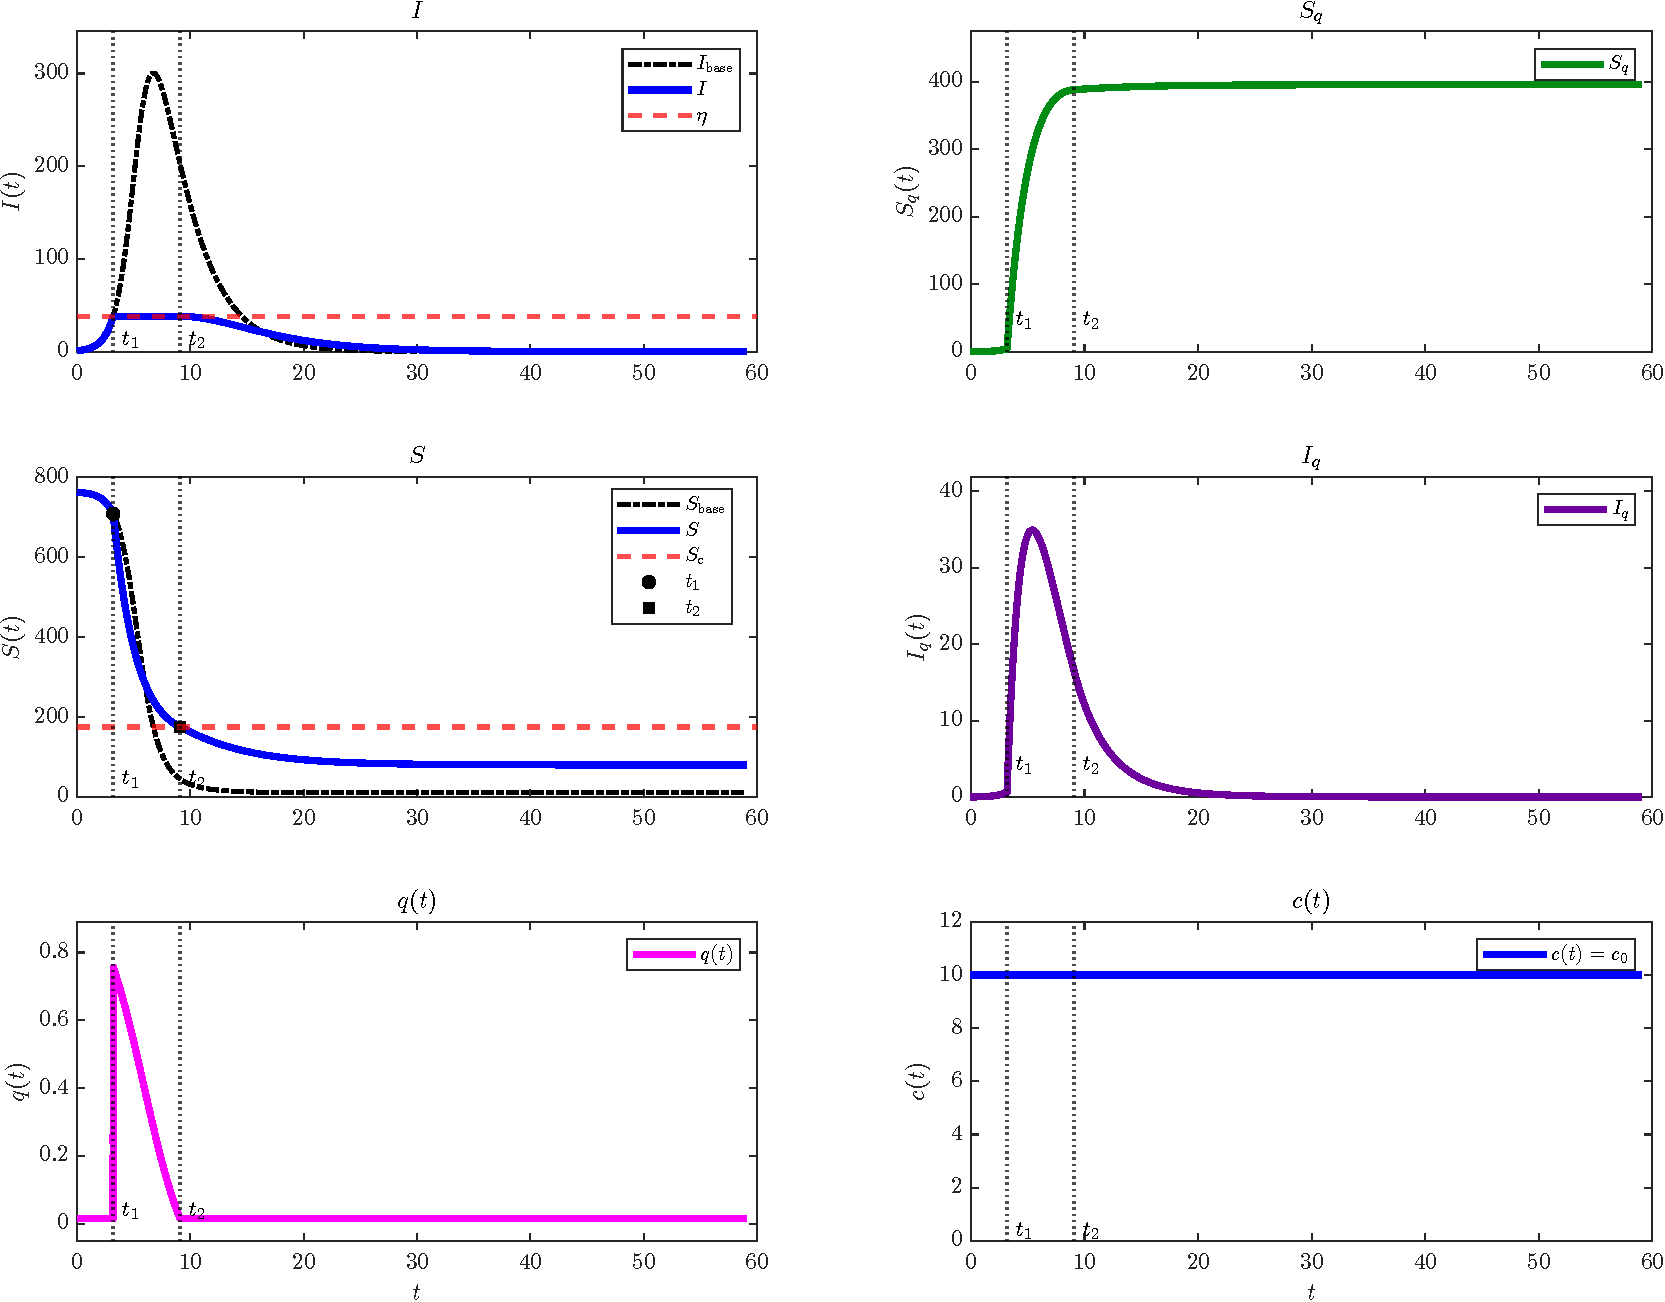
\includegraphics[width=0.7\textwidth]{figures/optimal_control_with_quarantine_panels.pdf}
    \label{fig:scenario1:single-sim}
\end{figure}

\begin{table}[htbp]
  \centering
  \footnotesize
  \caption{情景一数值模拟中的参数、理论结果与数值验证}
  \label{tab:results}
  \renewcommand{\arraystretch}{1.18}
  \setlength{\tabcolsep}{6pt}
  \begin{tabular}{llcllc}
    \toprule
    \multicolumn{6}{c}{\textbf{模型参数}} \\
    \midrule
    $\gamma$ & 0.3504 & \quad & $R_0$ & 4.3560 & \\
    $\beta$  & 0.1550 & \quad & $c_0$ & 10.0000 & \\
    $N$      & 763.0000 & \quad & $q_0$ & 0.0153 & \\
    $\eta$   & 38.1500 & \quad & $S_c$ & 175.1602 & \\
    $S_0$    & 762.0000 & \quad & $I_0$ & 1.0000 & \\
    \midrule

    \multicolumn{6}{c}{\textbf{理论结果}} \\
    \midrule
    切入点 & \multicolumn{2}{l}{$S^*=708.3470$}
    & 启动时间 & \multicolumn{2}{l}{$t_1=3.1754$ 天} \\
    解除时间 & \multicolumn{2}{l}{$t_2=9.0780$ 天}
    & 控制时长 & \multicolumn{2}{l}{$\Delta t=5.9026$ 天} \\
    最大隔离率 & \multicolumn{2}{l}{$q_c(t_1)=0.7565$}
    & 终点隔离强度 & \multicolumn{2}{l}{$q_c(t_2)=q_0=0.0153$} \\
    \midrule

    \multicolumn{6}{c}{\textbf{数值峰值}} \\
    \midrule
    受控情形
    & \multicolumn{2}{l}{$\max I(t)=38.1500$}
    & 平台误差
    & \multicolumn{2}{l}{$\max_{[t_1,t_2]}|I-\eta|=1.07\times10^{-7}$} \\
    常规控制情形
    & \multicolumn{2}{l}{$\max I(t)=300.3726$}
    & 峰值时间
    & \multicolumn{2}{l}{$t=6.7065$ 天} \\
    \bottomrule
  \end{tabular}
\end{table}
为了进一步考察参数对情景一控制策略的影响，我们进行数值分析。与前述理论分析一致，本节重点考察两个政策参数 $c_0$ 与 $\eta$。第一组数值实验固定 $\beta,\gamma,q_0,N,S_0,I_0,\eta$，改变常规接触水平 $c_0$；第二组数值实验固定 $\beta,\gamma,c_0,q_0,N,S_0,I_0$，改变医疗容量阈值 $\eta$。对基准阈值 $\eta=0.05N$，由式~\eqref{eq:s1:c0-min-equality} 数值求得
\[
c_{0,\min}(0.05N)\approx3.3270.
\]
因此，$c_0$ 的一维扫描从 $c_{0,\min}+0.02\approx3.3470$ 开始，而不再只考察 $c_0\geq6$ 的下降分支。对每组参数，程序首先判断系统在常规防控背景下是否能够触及 $I=\eta$。若可行，则输出切入点 $S^*$、常规防控临界阈值 $S_c$、启动时间 $t_1$、控制时长 $\Delta t$、启动时刻所需最大隔离率
\[
q_{\max}=q_c(t_1),
\]
清零时间 $t_{\rm end}$，以及综合成本 $J$ 和总累计感染 $I_{t_{\rm cum}}$。相应的数值结果见表~\ref{tab:scenario1_c0_summary}--\ref{tab:scenario1_eta_summary} 和图~\ref{fig:scenario1_u_time_c0}--\ref{fig:scenario1_feasibility_c0_eta}。

\begin{table}[htbp]
  \centering
  \footnotesize
  \caption{情景一中不同 $c_0$ 下的关键控制指标。}
  \label{tab:scenario1_c0_summary}
  \begin{tabular}{ccccccccc}
\toprule
$c_0$ & $S^*$ & $S_c$ & $t_1$ & $\Delta t$ & $t_{\rm end}$ & $q_{\max}$ & $J$ & $I_{t_{\rm cum}}$ \\
\midrule
3.347 & 559.1496 & 523.3306 & 29.9176 & 2.0432 & 71.4690 & 0.0783 & 0.0053 & 382.5525 \\
3.5 & 608.8267 & 500.4576 & 23.6110 & 4.7339 & 67.0709 & 0.1905 & 0.0897 & 374.1316 \\
4 & 654.6273 & 437.9004 & 15.3697 & 6.8658 & 58.7277 & 0.3413 & 0.4374 & 360.7318 \\
4.5 & 672.5044 & 389.2448 & 11.5687 & 7.4407 & 53.6541 & 0.4300 & 0.7690 & 351.1079 \\
5 & 682.5742 & 350.3203 & 9.3039 & 7.5778 & 49.9657 & 0.4946 & 1.0561 & 342.5629 \\
5.5 & 689.1189 & 318.4730 & 7.7894 & 7.5305 & 47.0633 & 0.5449 & 1.2973 & 334.7234 \\
6 & 693.7367 & 291.9336 & 6.7023 & 7.3965 & 44.6748 & 0.5856 & 1.4974 & 327.4892 \\
7 & 699.8442 & 250.2288 & 5.2432 & 7.0279 & 40.9038 & 0.6479 & 1.7981 & 314.6222 \\
8 & 703.7125 & 218.9502 & 4.3073 & 6.6308 & 38.0095 & 0.6936 & 2.0006 & 303.5829 \\
9 & 706.3866 & 194.6224 & 3.6556 & 6.2514 & 35.6892 & 0.7287 & 2.1355 & 294.0417 \\
10 & 708.3470 & 175.1602 & 3.1754 & 5.9026 & 33.7732 & 0.7565 & 2.2236 & 285.7244 \\
11 & 709.8463 & 159.2365 & 2.8069 & 5.5863 & 32.1563 & 0.7791 & 2.2789 & 278.4115 \\
12 & 711.0304 & 145.9668 & 2.5150 & 5.3007 & 30.7687 & 0.7978 & 2.3110 & 271.9295 \\
13 & 711.9893 & 134.7386 & 2.2782 & 5.0428 & 29.5616 & 0.8136 & 2.3263 & 266.1413 \\
\bottomrule
\end{tabular}

\end{table}

\begin{table}[htbp]
  \centering
  \footnotesize
  \caption{情景一中不同 $\eta$ 下的关键控制指标。}
  \label{tab:scenario1_eta_summary}
  \begin{tabular}{cccccccccc}
\toprule
$\eta$ & $\eta/N$ & $S^*$ & $S_c$ & $t_1$ & $\Delta t$ & $t_{\rm end}$ & $q_{\max}$ & $J$ & $I_{t_{\rm cum}}$ \\
\midrule
15.26 & 0.02 & 741.5490 & 175.1602 & 2.3459 & 15.0431 & 46.8029 & 0.7674 & 5.8888 & 233.7810 \\
19.07 & 0.025 & 736.0485 & 175.1602 & 2.5437 & 11.9974 & 42.7594 & 0.7657 & 4.6678 & 243.9840 \\
22.89 & 0.03 & 730.5351 & 175.1602 & 2.7070 & 9.9665 & 39.9267 & 0.7639 & 3.8536 & 253.3432 \\
26.71 & 0.035 & 725.0086 & 175.1602 & 2.8464 & 8.5156 & 37.8161 & 0.7621 & 3.2718 & 262.0776 \\
30.52 & 0.04 & 719.4686 & 175.1602 & 2.9684 & 7.4271 & 36.1746 & 0.7603 & 2.8353 & 270.3267 \\
34.34 & 0.045 & 713.9148 & 175.1602 & 3.0771 & 6.5803 & 34.8569 & 0.7584 & 2.4955 & 278.1861 \\
38.15 & 0.05 & 708.3470 & 175.1602 & 3.1754 & 5.9026 & 33.7732 & 0.7565 & 2.2236 & 285.7244 \\
\bottomrule
\end{tabular}

\end{table}

\begin{figure}[htbp]
    \centering
    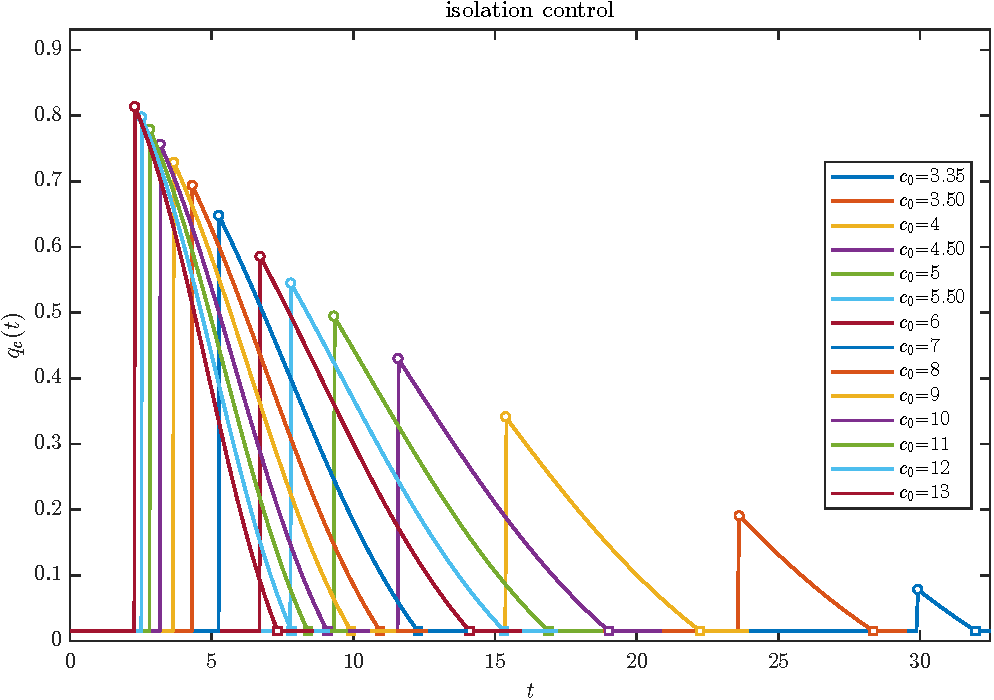
\includegraphics[width=0.72\textwidth]{figures/scenario1_u_time_c0.pdf}
    \caption{情景一中不同 $c_0$ 下隔离率 $q_c(t)$ 的时间轨迹。}
    \label{fig:scenario1_u_time_c0}
\end{figure}

\begin{figure}[htbp]
    \centering
    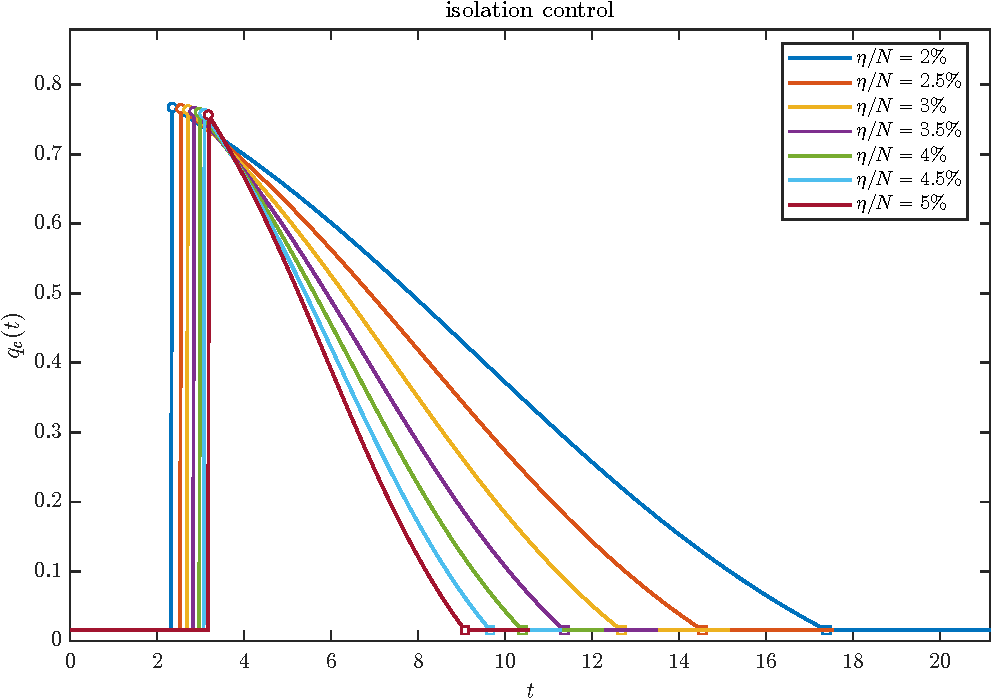
\includegraphics[width=0.72\textwidth]{figures/scenario1_u_time_eta.pdf}
    \caption{情景一中不同 $\eta$ 下隔离率 $q_c(t)$ 的时间轨迹。}
    \label{fig:scenario1_u_time_eta}
\end{figure}

\begin{figure}[htbp]
    \centering
    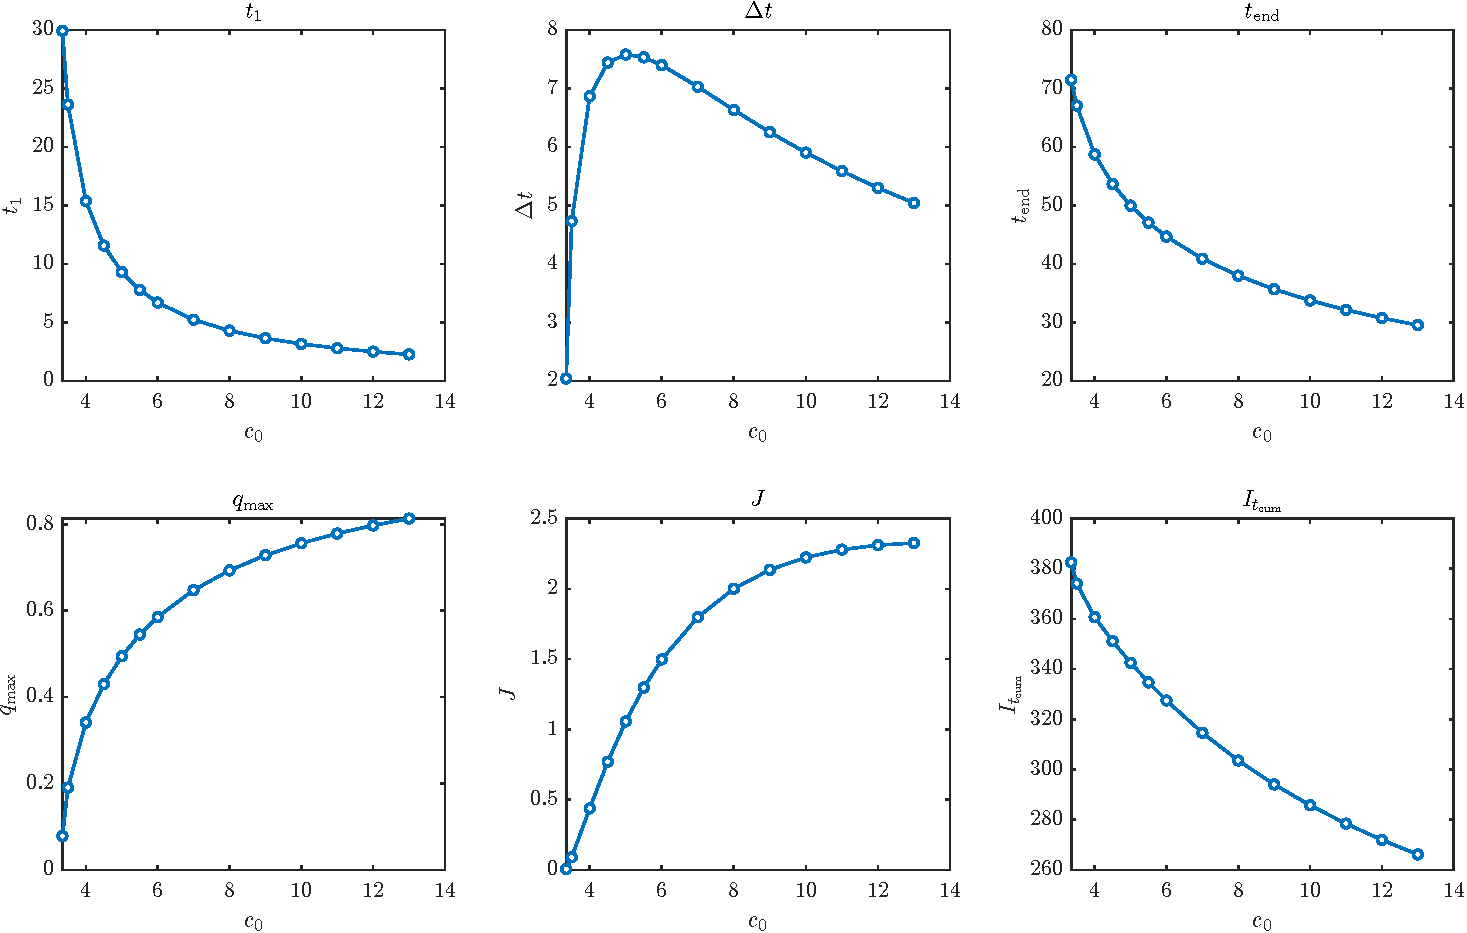
\includegraphics[width=0.88\textwidth]{figures/scenario1_summary_c0.pdf}
    \caption{情景一中关键指标随 $c_0$ 的变化，其中扫描范围从 $c_{0,\min}+0.02$ 延伸至 $13$。}
    \label{fig:scenario1_summary_c0}
\end{figure}

\begin{figure}[htbp]
    \centering
    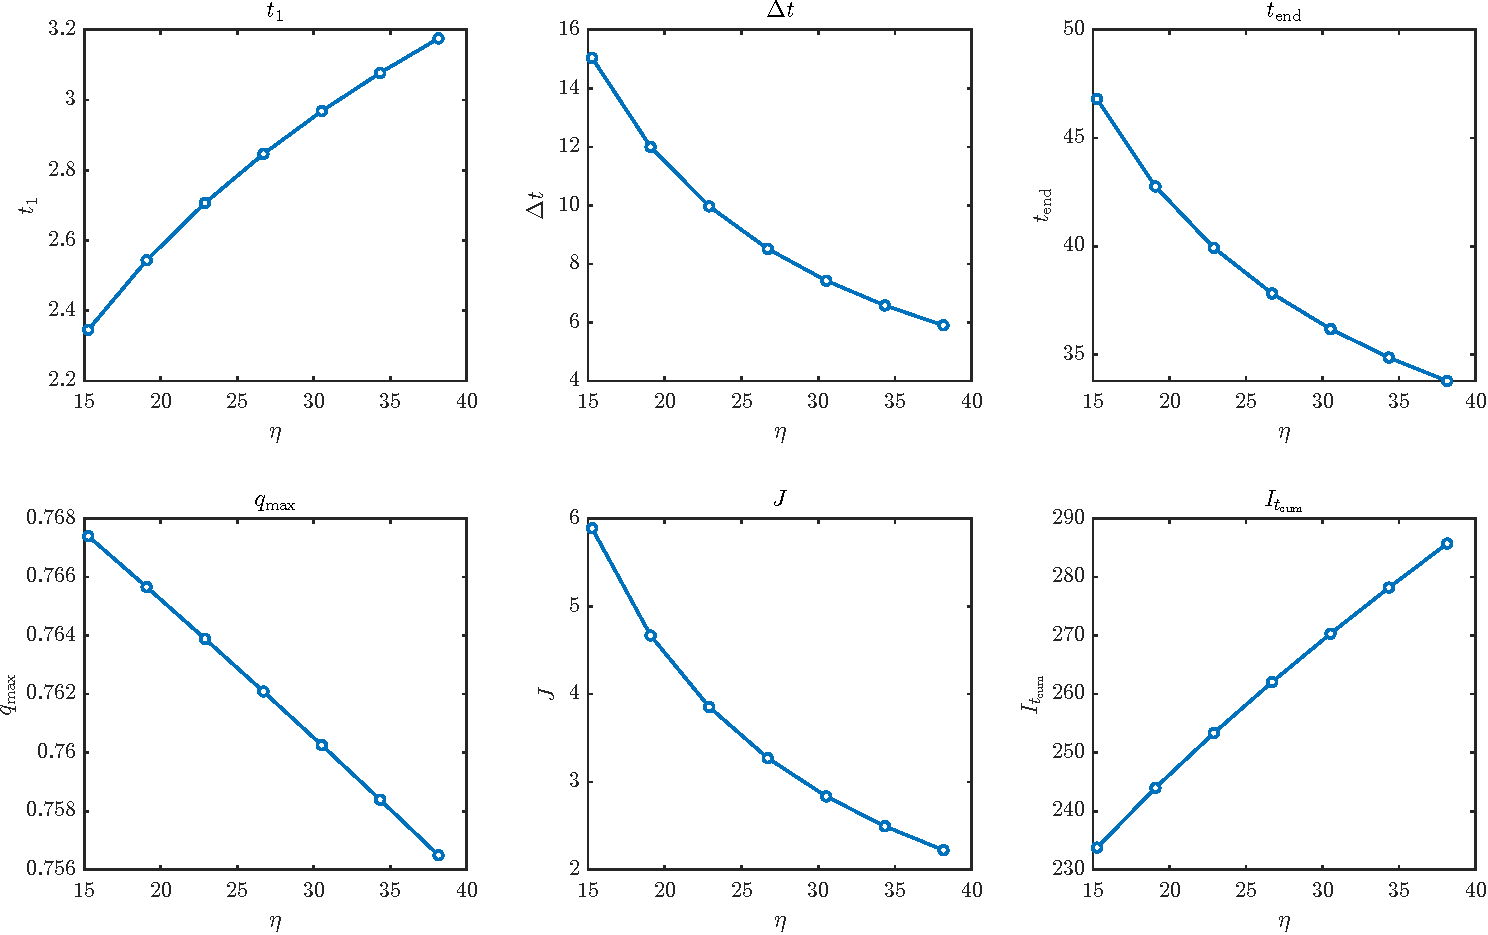
\includegraphics[width=0.88\textwidth]{figures/scenario1_summary_eta.pdf}
    \caption{情景一中关键指标随 $\eta$ 的变化。}
    \label{fig:scenario1_summary_eta}
\end{figure}

\begin{figure}[htbp]
    \centering
    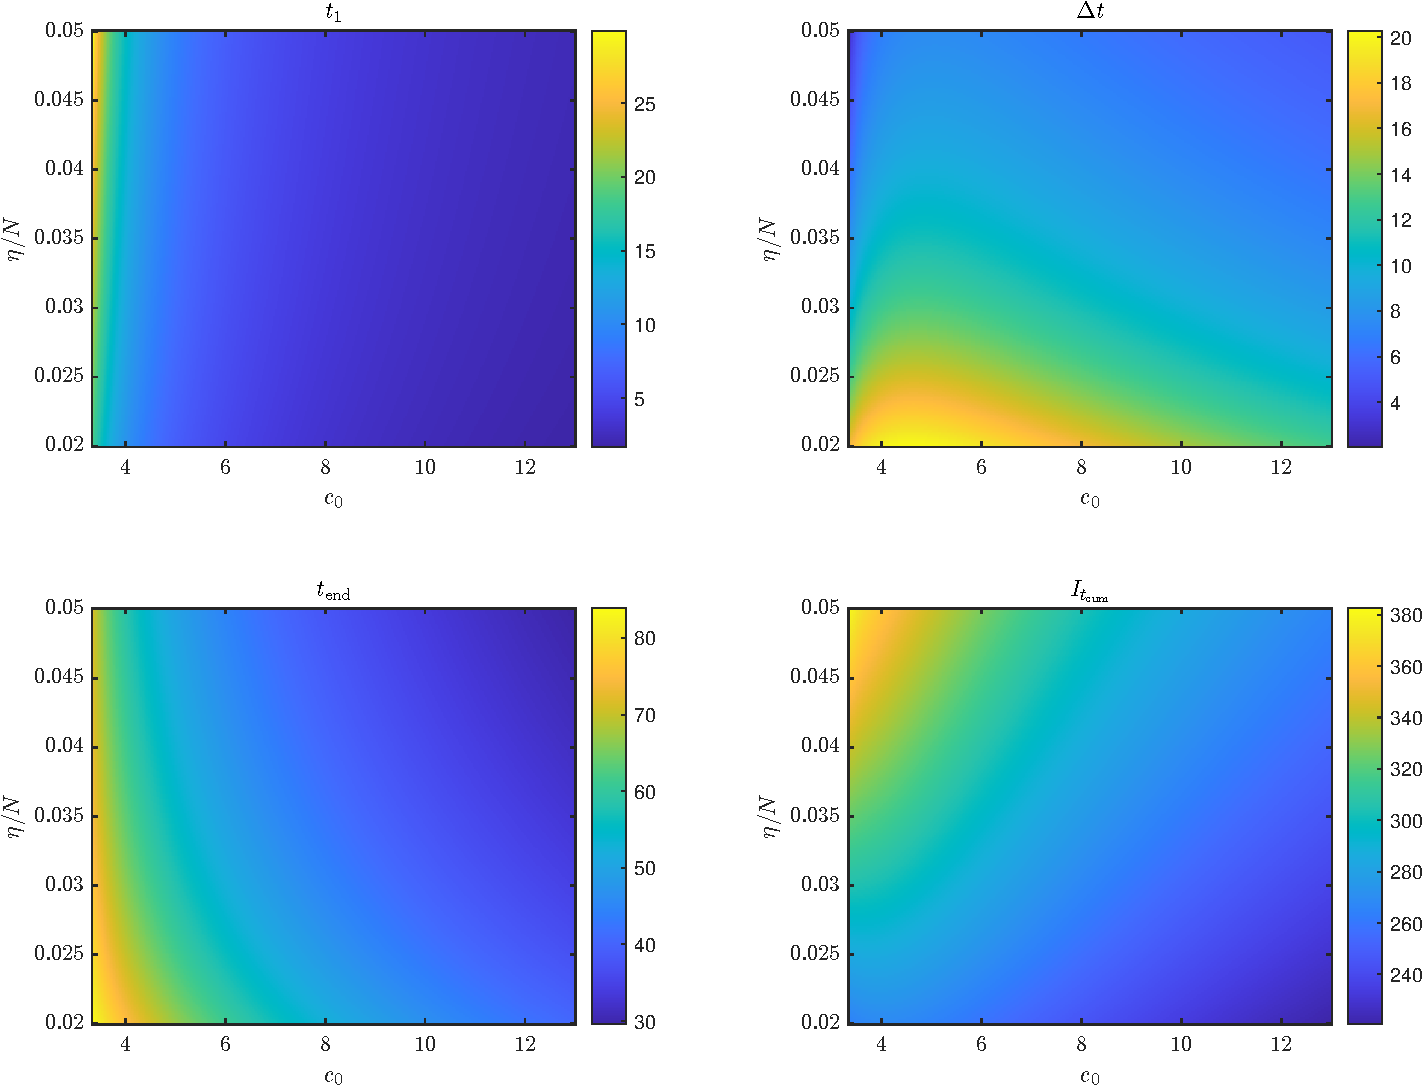
\includegraphics[width=0.88\textwidth]{figures/scenario1_heatmaps_c0_eta.pdf}
    \caption{情景一中 $(c_0,\eta)$ 平面上的 $t_1$、$\Delta t$、$t_{\rm end}$ 与 $I_{t_{\rm cum}}$ 热图。}
    \label{fig:scenario1_heatmaps_c0_eta}
\end{figure}

\begin{figure}[htbp]
    \centering
    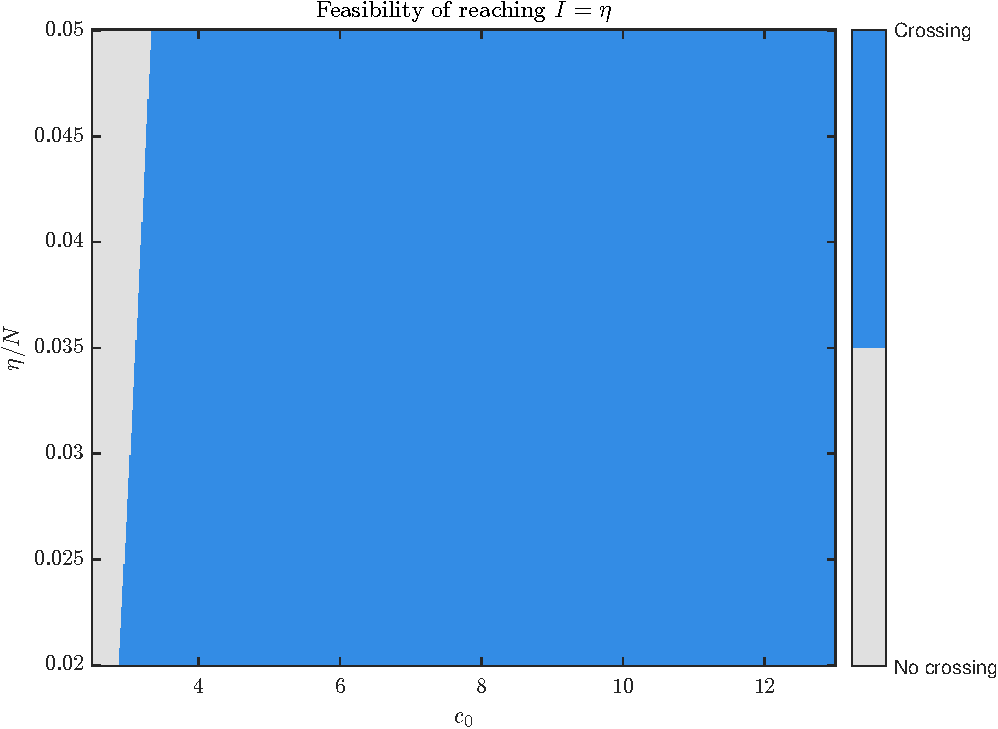
\includegraphics[width=0.68\textwidth]{figures/scenario1_feasibility_c0_eta.pdf}
    \caption{情景一中 $(c_0,\eta)$ 平面上是否能够触及 $I=\eta$ 的可行性区域。}
    \label{fig:scenario1_feasibility_c0_eta}
\end{figure}

从表~\ref{tab:scenario1_c0_summary} 和图~\ref{fig:scenario1_summary_c0} 可以看出，在固定 $\beta,\gamma,q_0,N,S_0,I_0,\eta$ 时，随着常规接触水平 $c_0$ 增大，系统触及医疗红线的时间 $t_1$ 明显提前，切入点 $S^*$ 上升，所需最大隔离率 $q_{\max}$ 增大。这与理论分析中 $S^*_{c_0}>0$、$t_{1,c_0}<0$ 以及 $q_{\max}$ 随 $c_0$ 增大而上升的结论一致。控制时长 $\Delta t$ 则呈现非单调变化：当 $c_0$ 从 $3.3470$ 增大到 $5$ 时，$\Delta t$ 从 $2.0432$ 天增加到 $7.5778$ 天；此后随着 $c_0$ 继续增大，$\Delta t$ 逐渐下降，在 $c_0=13$ 时为 $5.0428$ 天。当前离散扫描的最大值出现在 $c_0=5$，这表明转折点位于其附近，但该离散点不作为解析极值位置。该结果同时展示了式~\eqref{eq:s1:c0-min-limit} 所给出的左端边界趋势以及导数判别式允许的正、负两个分支。清零时间 $t_{\rm end}$、成本 $J$ 和总累计感染 $I_{t_{\rm cum}}$ 还受到控制后衰减阶段和累计流量的影响，不能由 $\Delta t$ 的变化方向直接推出。

从表~\ref{tab:scenario1_eta_summary} 和图~\ref{fig:scenario1_summary_eta} 可以看出，在固定 $c_0$ 的情况下，医疗容量阈值 $\eta$ 越高，系统越晚触碰红线，即 $t_1$ 增大；触碰时易感者已经消耗更多，因此 $S^*$ 下降。与此同时，控制持续时间 $\Delta t$、最大隔离率 $q_{\max}$ 以及成本 $J$ 均下降。这与理论分析中 $S^*_\eta<0$、$t_{1,\eta}>0$、$\Delta t_\eta<0$ 以及 $q_{\max,\eta}<0$ 的结论一致。清零时间 $t_{\rm end}$ 和总累计感染 $I_{t_{\rm cum}}$ 同时受到平台高度、平台时长和后期衰减阶段的共同影响，因此在数值结果中单独列出。

图~\ref{fig:scenario1_u_time_c0}--\ref{fig:scenario1_u_time_eta} 展示不同参数组在时间轴上启动、维持和解除加强隔离的全过程。本文对参数敏感性的判断主要依据 $S^*$、$t_1$、$\Delta t$、$t_{\rm end}$、$q_{\max}$、$J$ 和 $I_{t_{\rm cum}}$。最后，图~\ref{fig:scenario1_heatmaps_c0_eta} 和图~\ref{fig:scenario1_feasibility_c0_eta} 给出了 $(c_0,\eta)$ 平面上的关键指标变化与可行性区域，进一步说明当医疗容量较高或常规传播强度较低时，系统可能不会触及医疗红线，从而无需启动加强隔离控制。





\section{西安控制比较预留章节}
本节预留给西安疫情数据下的 TDINN控制、情景一阈值控制和常规控制比较。后续合并时，符号统一使用 $I_{\rm new}(t)$、$I_{q_{\rm new}}(t)$、$I_{\rm cum}(t)$、$I_{q_{\rm cum}}(t)$ 和 $I_{t_{\rm cum}}(t)$；图表标签统一使用 \texttt{xian} 命名空间，以避免和前文理论标签冲突。



\section{单阈值响应图谱预留章节}
本节预留给单阈值控制响应图谱、二次加权成本和 $(\eta,c_0)$ 二维敏感性分析。后续合并时，低阈值结果作为长期低感染水平维持或常态化管控的数学情形处理，不直接替换西安主基准结果。

\section{情景二：全程固定$q(t) \equiv q_0$,只用$c(t)$控制}

\section{情景三：同时调节$c(t)$和$q(t)$}



\end{document}

